%!TEX root = ../../dissertation.tex


\section{Rosetta} % (fold)
\label{sec:rosetta}
Rosetta \cite{lopes2011portable} is a tool for \gls{GD} that was created with very specific goals. The focus users are designers and architects, that usually do not have programming experience. So the goals was to be pedagogic, i.e. easy to learn, easy to use. To be capable to interact with the most used \gls{CAD} tools as back-ends and also implement several \glspl{PL} as front-ends.

\begin{figure}[htbp]
	\centering
	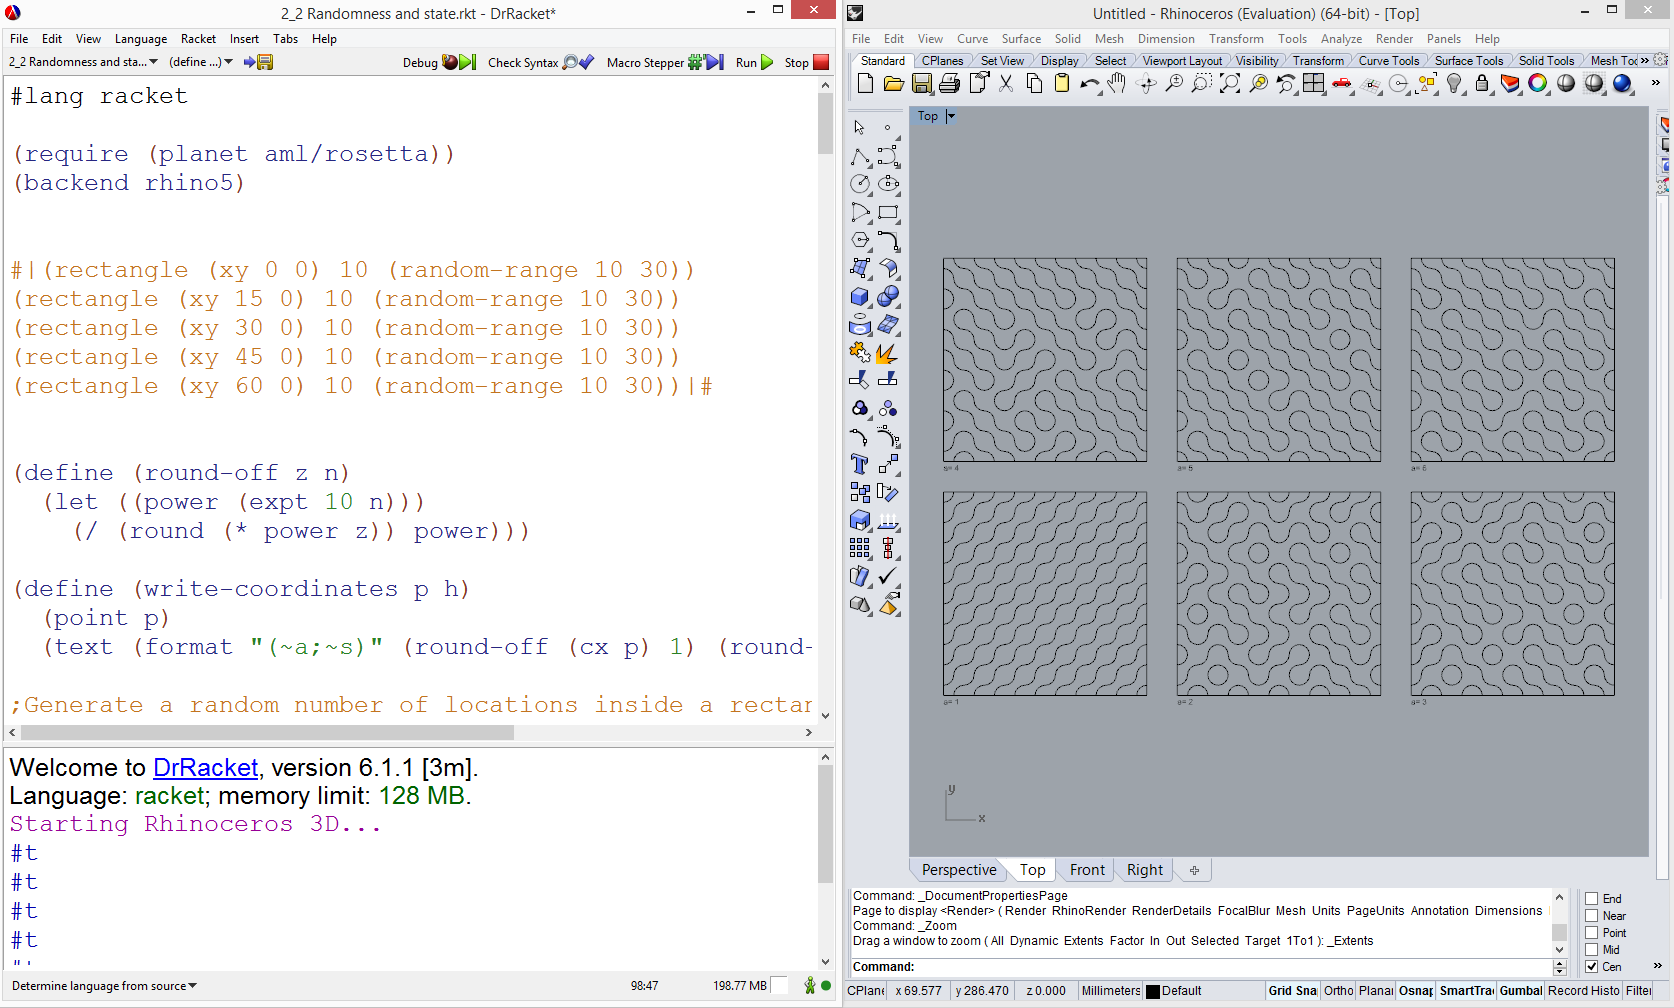
\includegraphics[width=0.95\textwidth]{images/Rosetta/Rosetta4.png}
	\caption{Rosetta IDE with Rhino}
	\label{fig:RosettaRhino}
\end{figure}

\subsection{CADs} % (fold)
\label{sub:cads}

Rosetta implements back-ends for the most used \gls{CAD} tools (Section~\ref{sub:cads}), such as AutoCad and Rhinoceros 3D. 

Since this tools where developed mainly for manual use and interaction, they have performance problems when dealing with the large amounts of geometry that tools such as Rosetta are able to generate.



% subsection cads (end)

\subsection{Visualization Library} % (fold)
\label{sub:visualization_library}

To deal with the performance problem, one extra backend was written. This backend is build using the \gls{VL} (Section~\ref{sec:vizualization_library}).

Since the \gls{VL} was created having performance as an important goal, this backend is a great improvement in what performance is concerned. It is much faster to visualize the models created within Rosetta.
This backend provides some user manual interaction, but is mostly the movement of the camera. It does not support manual modification of the model.

On the other hand, after some tests with this platform within Rosetta, the performance was not perfect yet, especially with large models. Since this project was abandoned by the author, it is not expected to have updates that would improve this issue, and also correct bugs or help with problems that are faced during the development of a tool such as Rosetta.


%Visualization

%Modeling

%Interaction

%Usability

% subsection visualization_library (end)
% section rosetta (end)

		